The proof of concept consists on building a numerical, two-dimensional simulation of the super-lens. Theoretically, paraxial beams incident on each individual ommatidium should focus light onto a single point. As shown in figure (\ref{fig:Superlens POC}), the design is not capable of obtaining free aberration on the system focal point. This is highly in part because the lenses in the first and third layer have spherical aberrations. In particular, the further their focal points the higher the aberration. Thus, a strict optimization is needed in order to obtained the desired results for this work. \\

\begin{figure}[H]
    \centering
    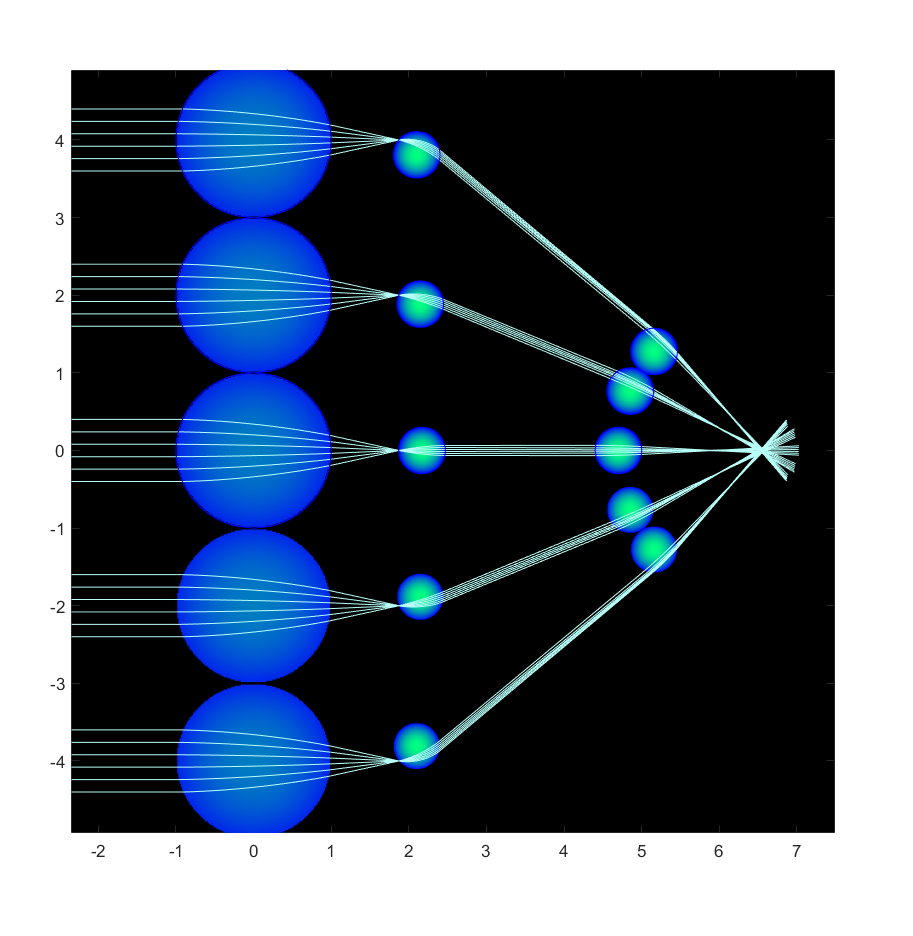
\includegraphics[width=\columnwidth]{Figures/MYSuperplens_POC.png}
    \caption{Two dimensional simulation of the proposed super-lens design to present the proof of concept.}
    \label{fig:Superlens POC}
\end{figure}


Also a three dimensional rendering is presented. With this design, the practical applications disused in the opening lines of the work can be exploited. 

\begin{figure}[H]
    \centering
    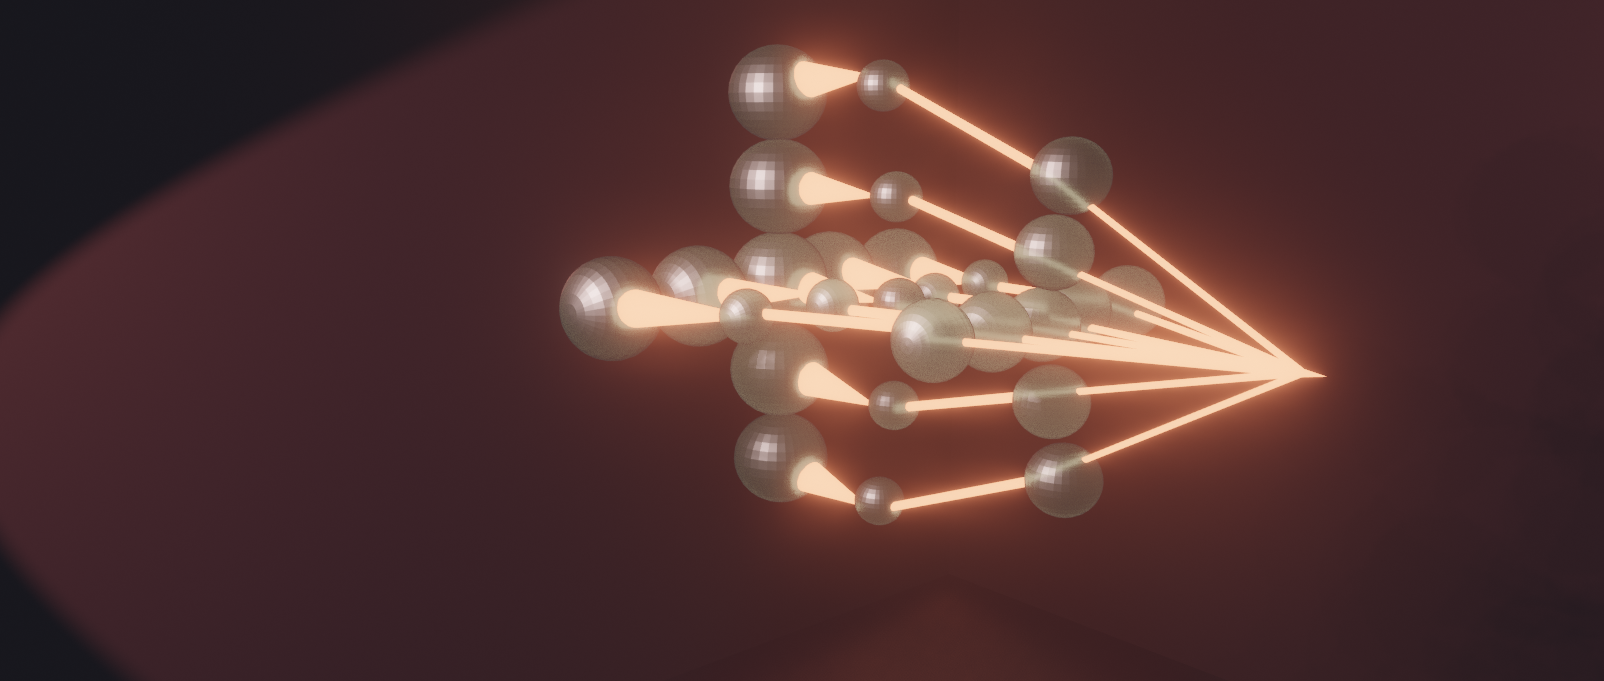
\includegraphics[width=\columnwidth]{Figures/Side-front-superlens.png}
    \caption{Three dimensional model of the proposed super-lens design.}
    \label{fig:Superlens design}
\end{figure}